\section{Harmonic distortion}

In this section the amount of harmonic distortion of the loudspeaker is analysed, to examine if it is possible to determine the performance of the loudspeaker from harmonics. To analyse the harmonic distortion a spectrogram is used. The spectrogram is a three dimensional plot which shows the frequency, time and magnitude. Basically the spectrogram is an array of multiple FFT each calculated at a given time with a given window.

The advantages of using a spectrogram is that it gives a good overview of the spectral content in the signal at any given time. Since the harmonic frequencies depends on the fundamental frequency, it is better to use a spectrogram rather than a regular FFT, since the spectrogram will reveal all harmonic distortion for all fundamental frequency from 10 Hz to 2.4 kHz. The spectrograms for microphone in dataset 1 and 19 are shown in \autoref{fig:spec_mic}.

\begin{figure}[H]
\centering
\begin{subfigure}[t]{0.47\textwidth}
	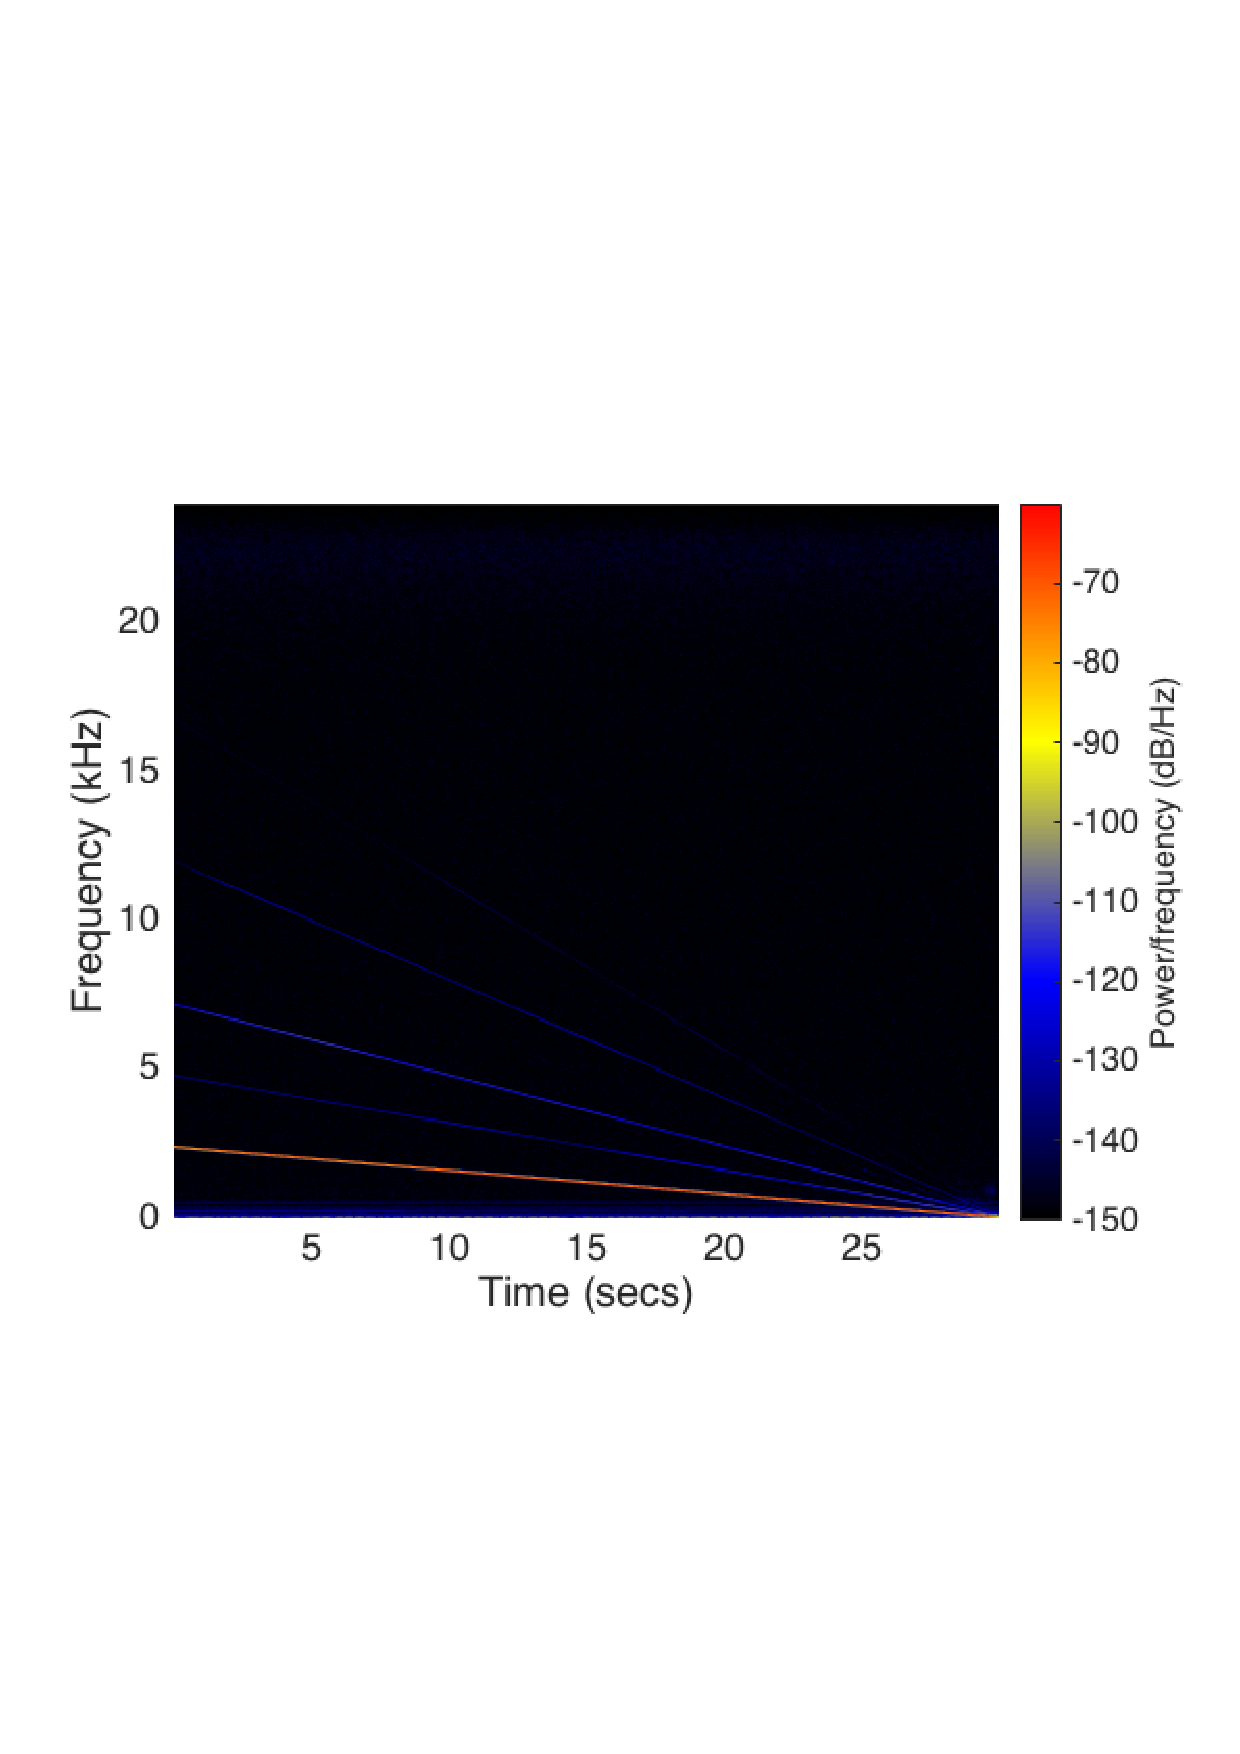
\includegraphics[width=1\textwidth]{figures/spectrogram_mic1.pdf}
	\caption{Microphone dataset 1.}
	\label{fig:spectrogram_mic1}
\end{subfigure}
\begin{subfigure}[t]{0.47\textwidth}
	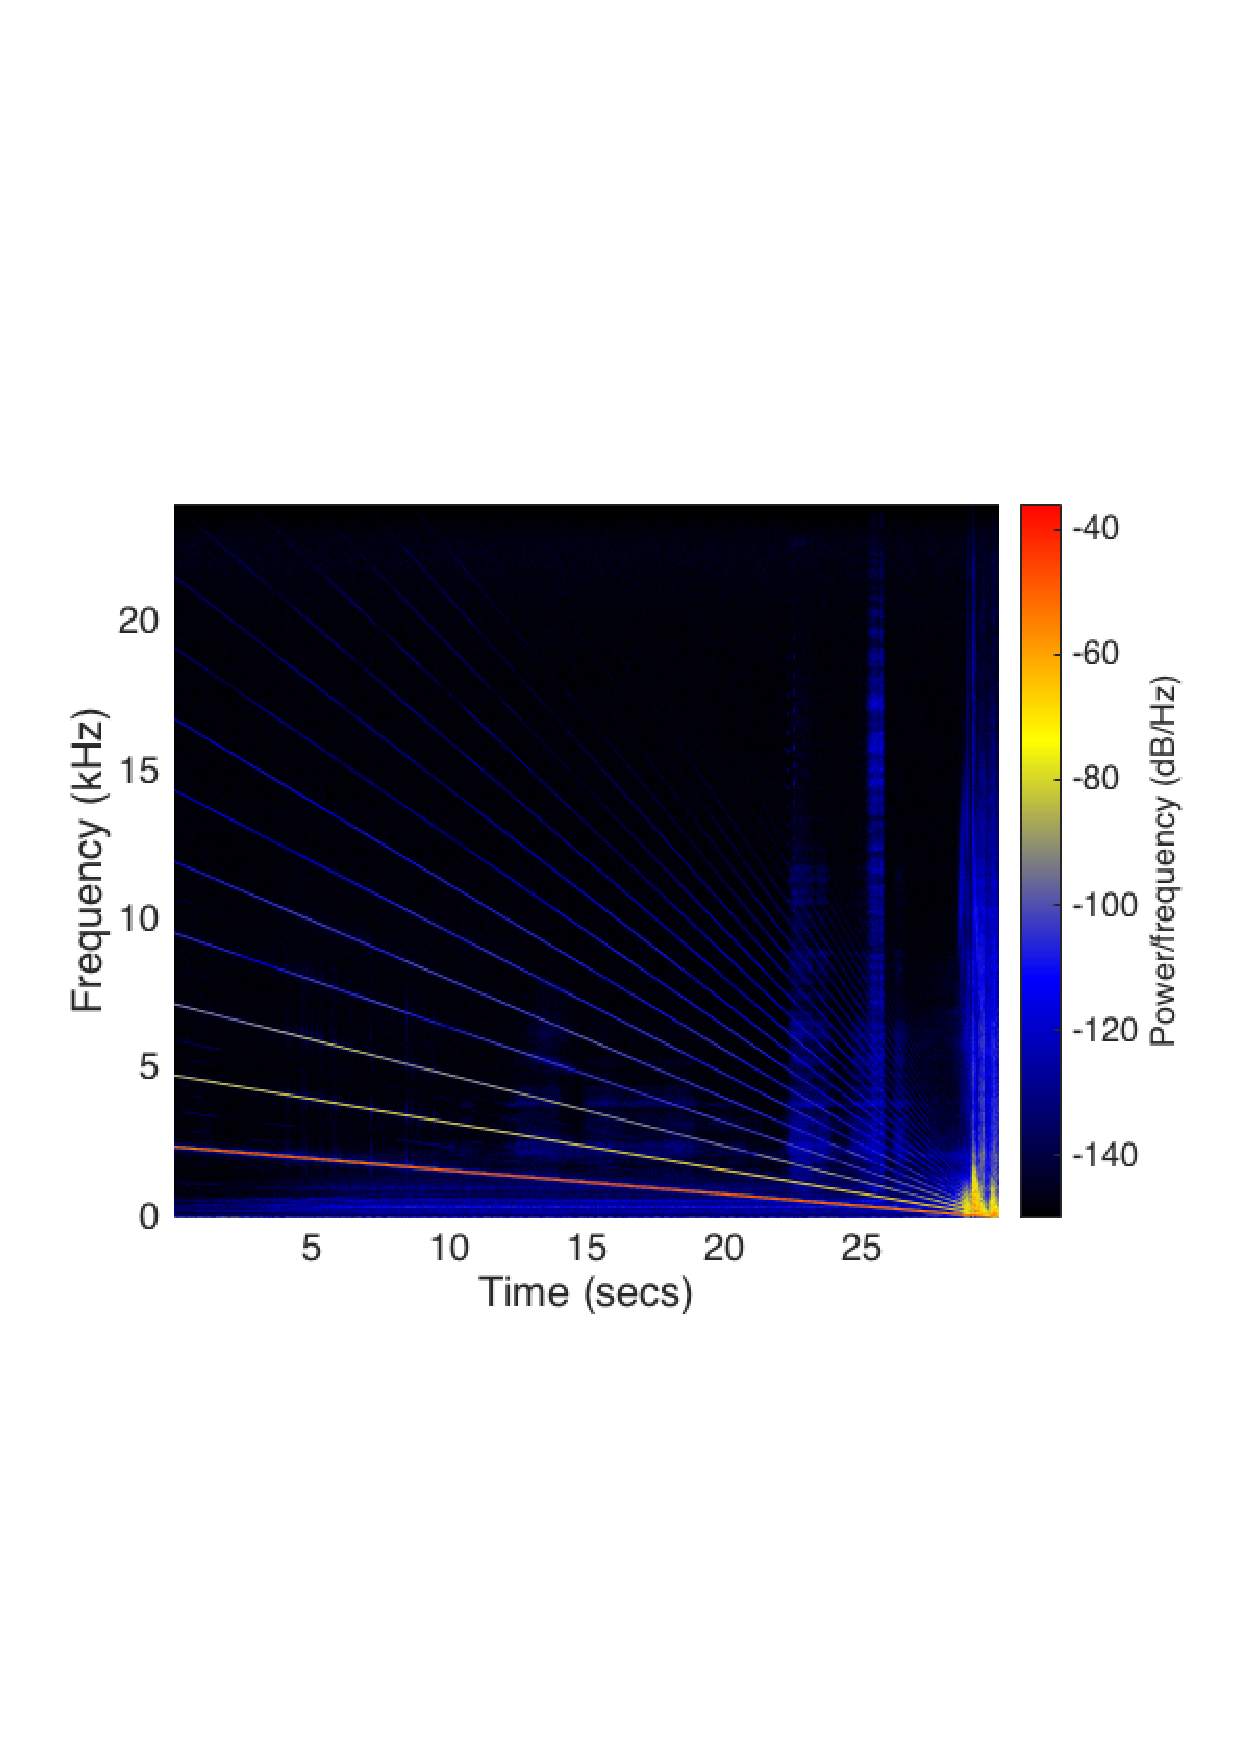
\includegraphics[width=1\textwidth]{figures/spectrogram_mic19.pdf}
	\caption{Microphone dataset 19.}
	\label{fig:spectrogram_mic19}
\end{subfigure}
\caption{The spectrograms of the microphone dataset 1 and 19. The prominent red line is the sine sweep from 2.4 kHz to 10 Hz while the yellow and blue lines along the red line are harmonic distortion.}
\label{fig:spec_mic}
\end{figure} 

The spectrograms of dataset 1 and 19 for the microphone, seen in \autoref{fig:spectrogram_mic1} and \autoref{fig:spectrogram_mic1}, show a prominent red line and three weak blue lines above the red line. It is seen that the red line is a linear decreasing function from 2.4 kHz to 10 Hz where the frequency is a function of time. This indicates that the red line is the fundamental frequency of the sine sweep from 2.4 kHz to 10 Hz. The blue and yellow line are linear functions of the harmonic distortions. The spectrograms clearly show that increasing the gain will increase the amount of harmonic distortion as well. An interesting observation is the spectral frequency leak that occurs at lower frequencies revealing large amount of distortion at low frequency and high gain. Since the power of the spectrum other than the harmonic frequencies increase, it could indicate that the coil hit the back plate of the driver at this point. From the analysis it can be concluded that the large amount of distortion can indicate that the coil is hitting the back plate of the driver.

The next part will be to analyse if similar observation can be found in the spectrogram for vibration measurements on the driver and the enclosure. 

\begin{figure}[H]
\centering
\begin{subfigure}[t]{0.47\textwidth}
	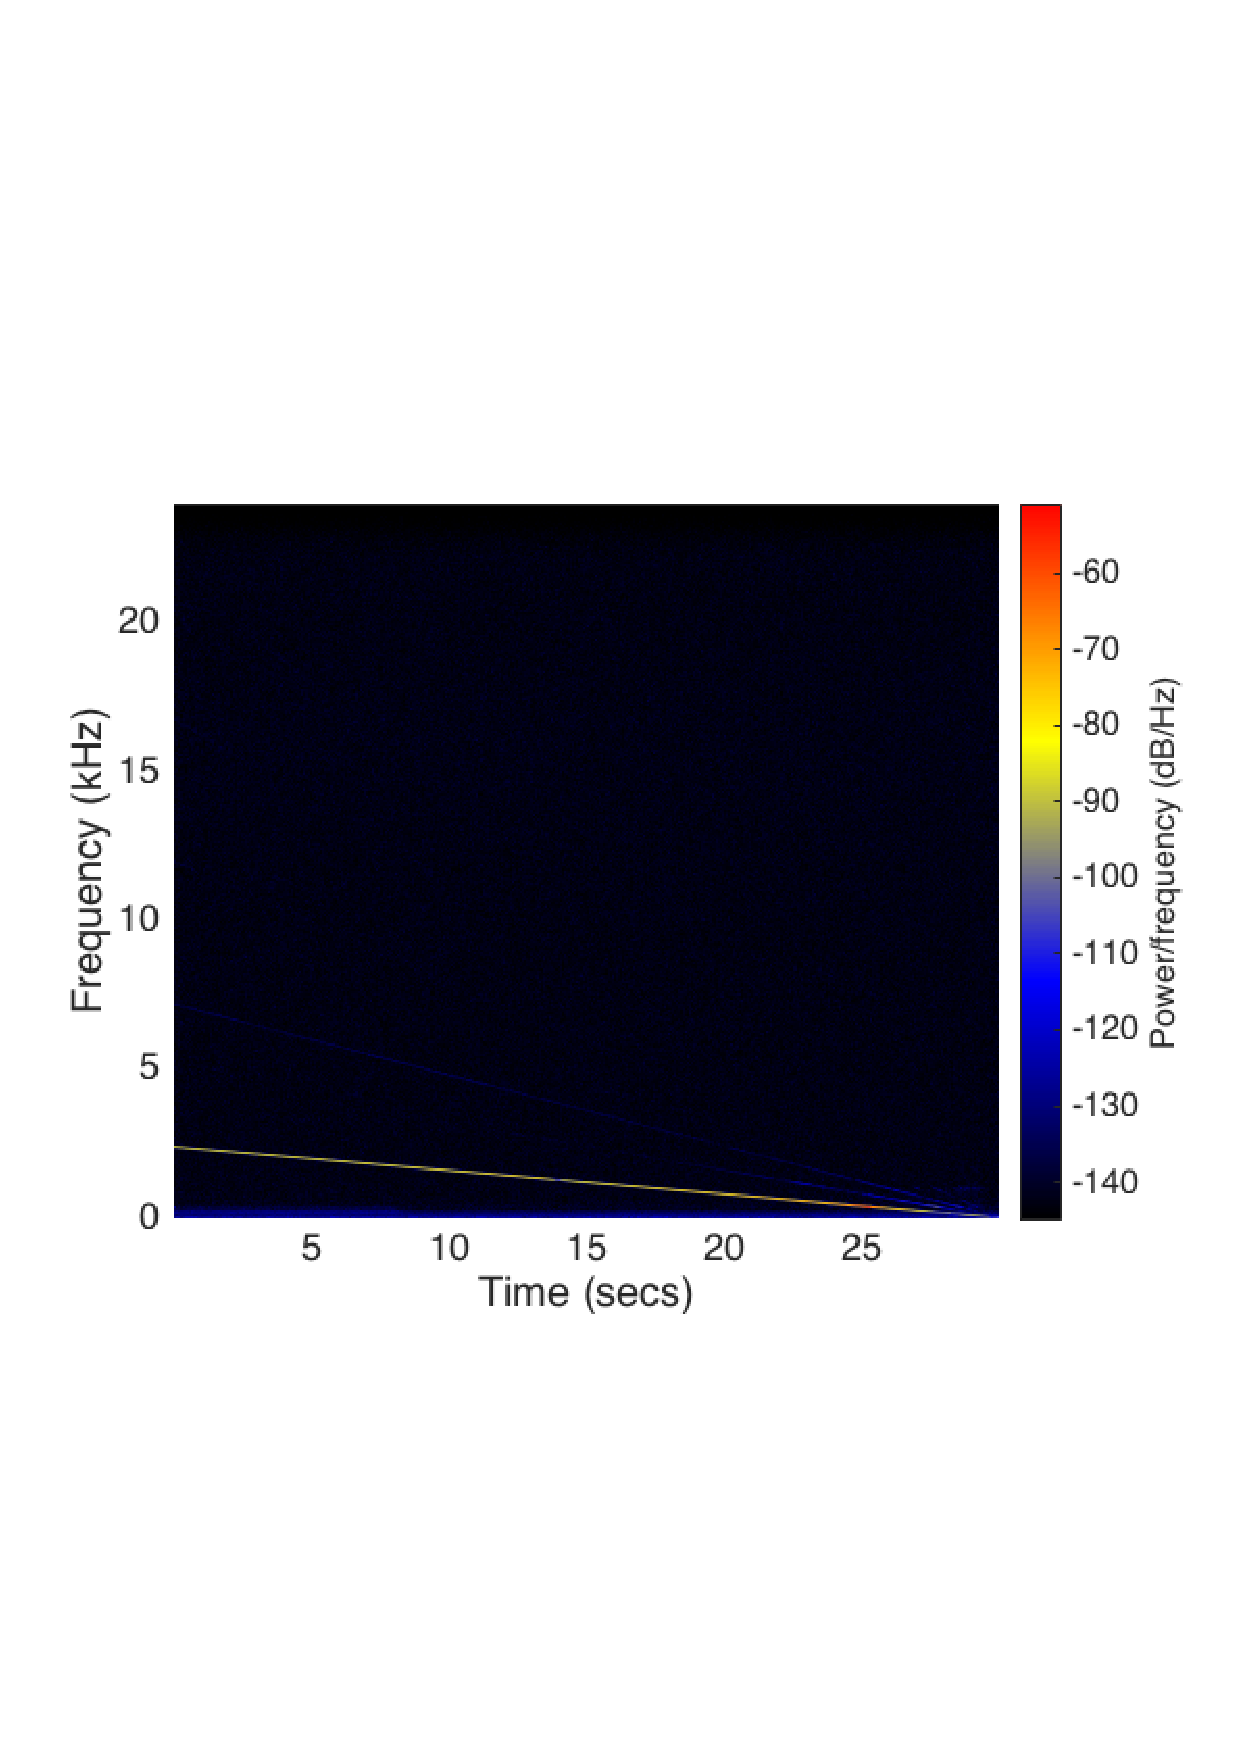
\includegraphics[width=1\textwidth]{figures/spectrogram_driver1.pdf}
	\caption{Driver dataset 1.}
	\label{fig:spectrogram_driver1}
\end{subfigure}
\begin{subfigure}[t]{0.47\textwidth}
	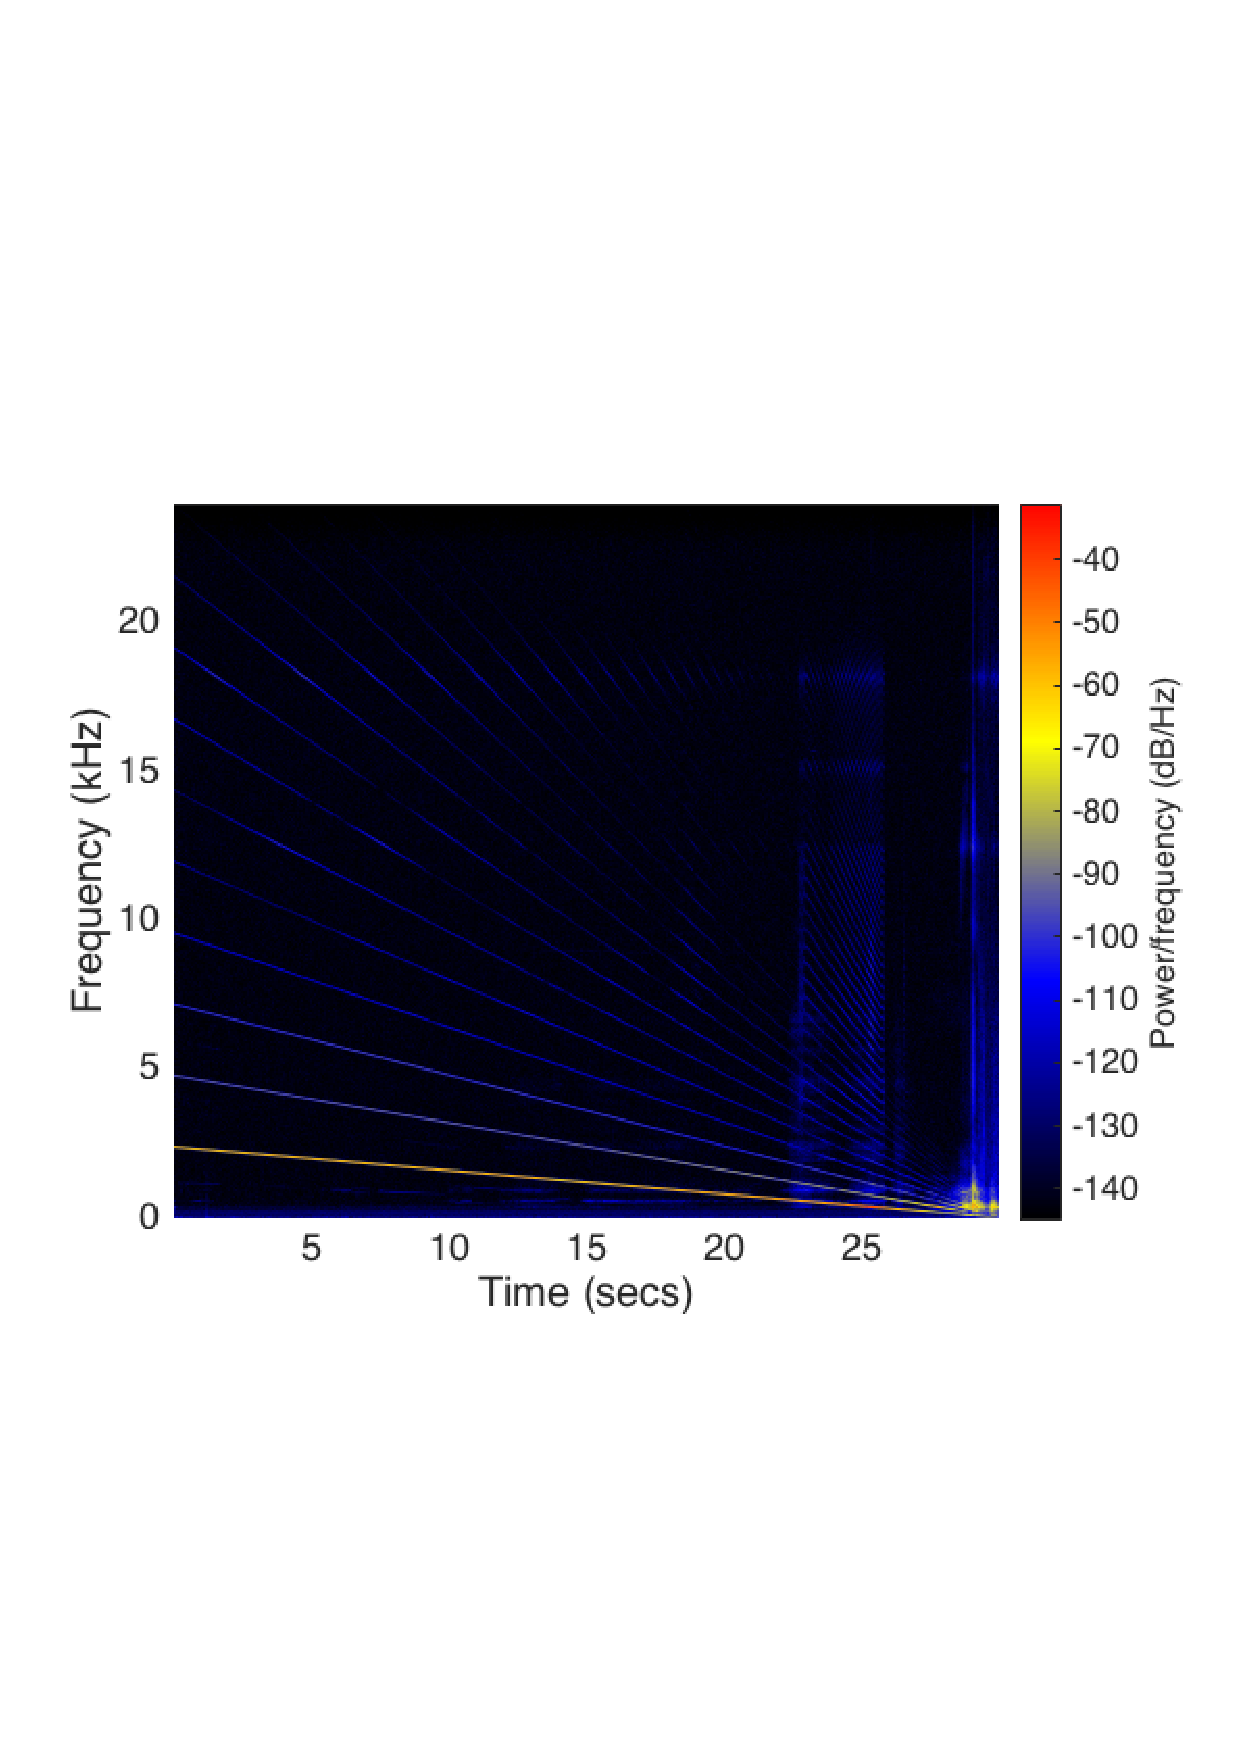
\includegraphics[width=1\textwidth]{figures/spectrogram_driver19.pdf}
	\caption{Driver dataset 19.}
	\label{fig:spectrogram_driver19}
\end{subfigure}
\caption{The spectrograms of the driver dataset 1 and 19. The prominent red line is the sine sweep from 2.4 kHz to 10 Hz while the yellow and blue lines along the red line are harmonic distortion.}
\label{fig:spec_driver}
\end{figure} 

The spectrograms of dataset 1 and 19 of the driver are seen in \autoref{fig:spec_driver}. From the spectrograms it is seen that the harmonic distortion is also present in the driver measurements as well as the frequency leak at lower frequencies at high gain. Finally the spectrum of the enclosure measurements is examined in \autoref{fig:spec_driver}.

\begin{figure}[H]
\centering
\begin{subfigure}[t]{0.47\textwidth}
	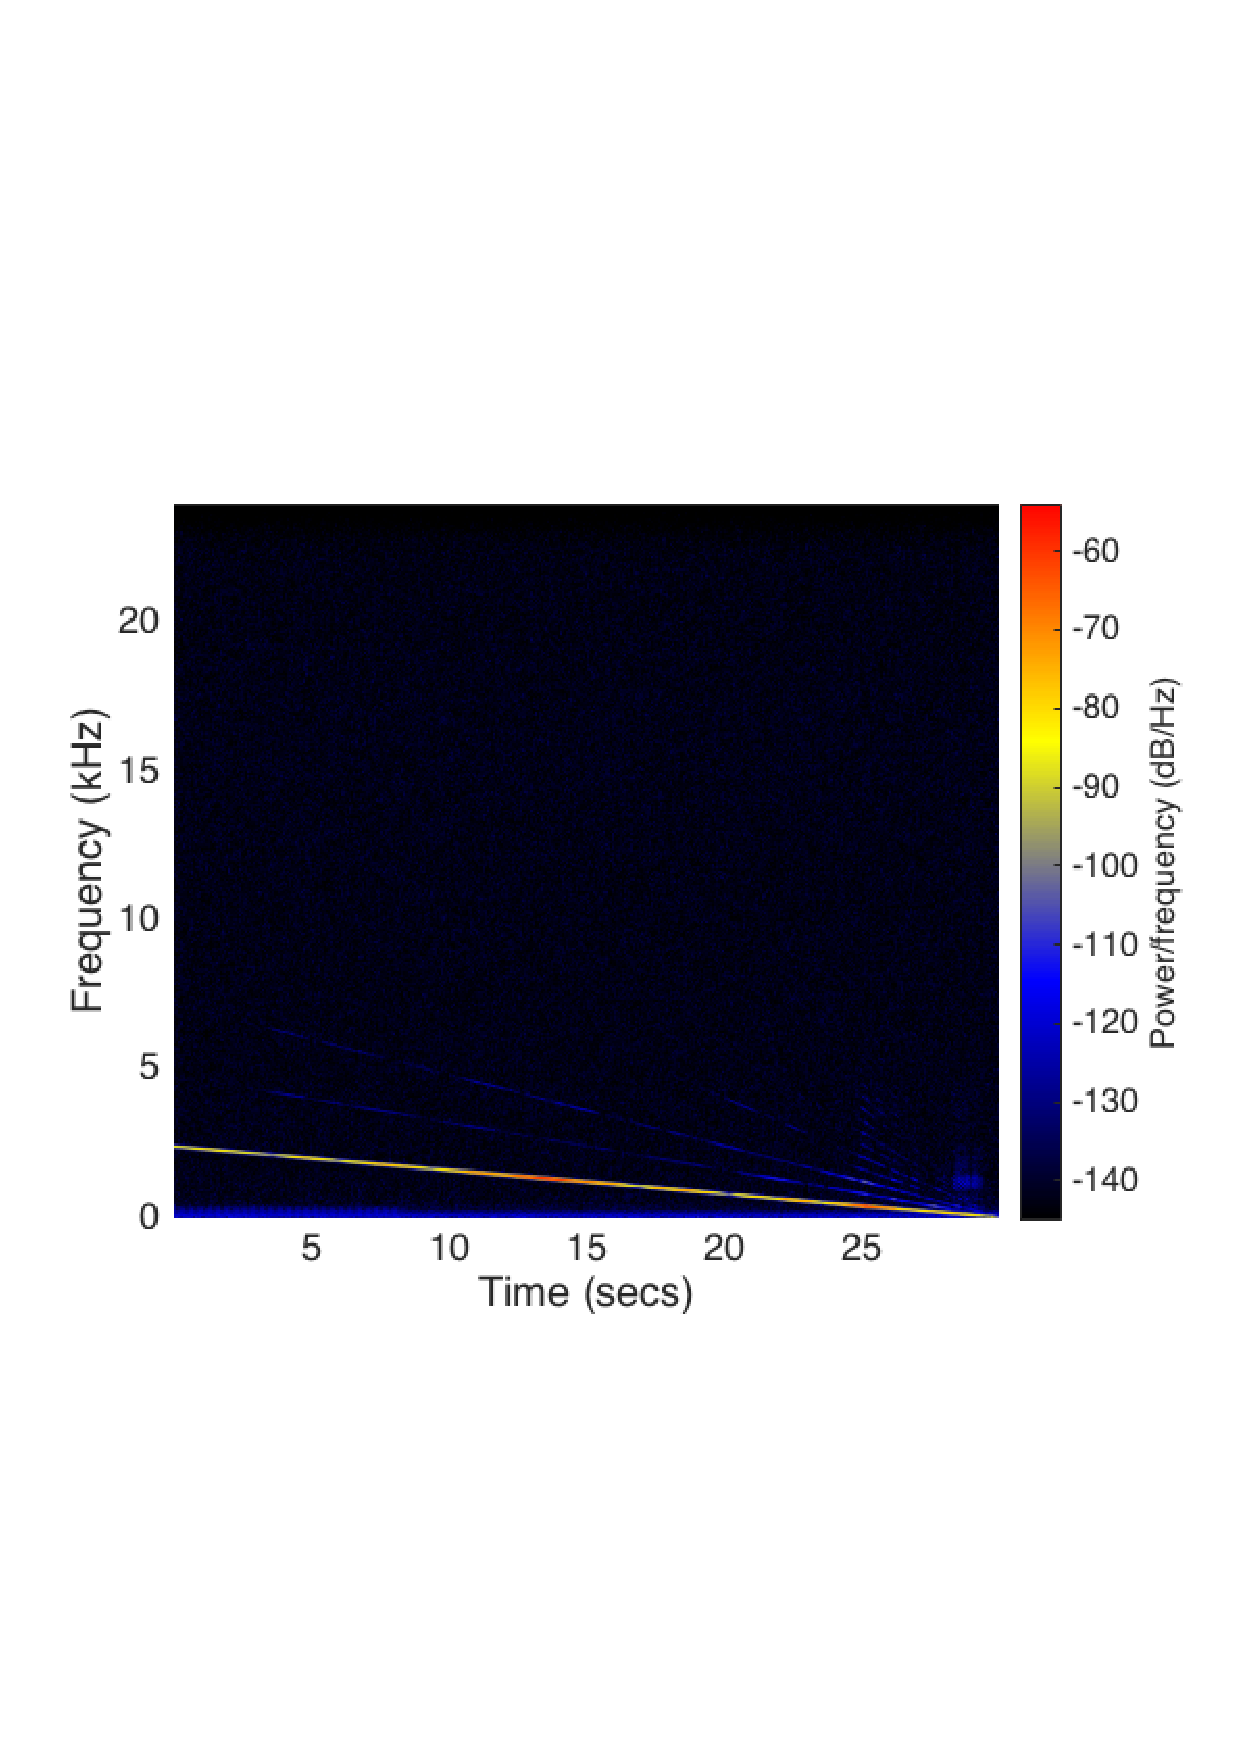
\includegraphics[width=1\textwidth]{figures/spectrogram_enclosure1.pdf}
	\caption{Enclosure dataset 1.}
	\label{fig:spectrogram_enclosure1}
\end{subfigure}
\begin{subfigure}[t]{0.47\textwidth}
	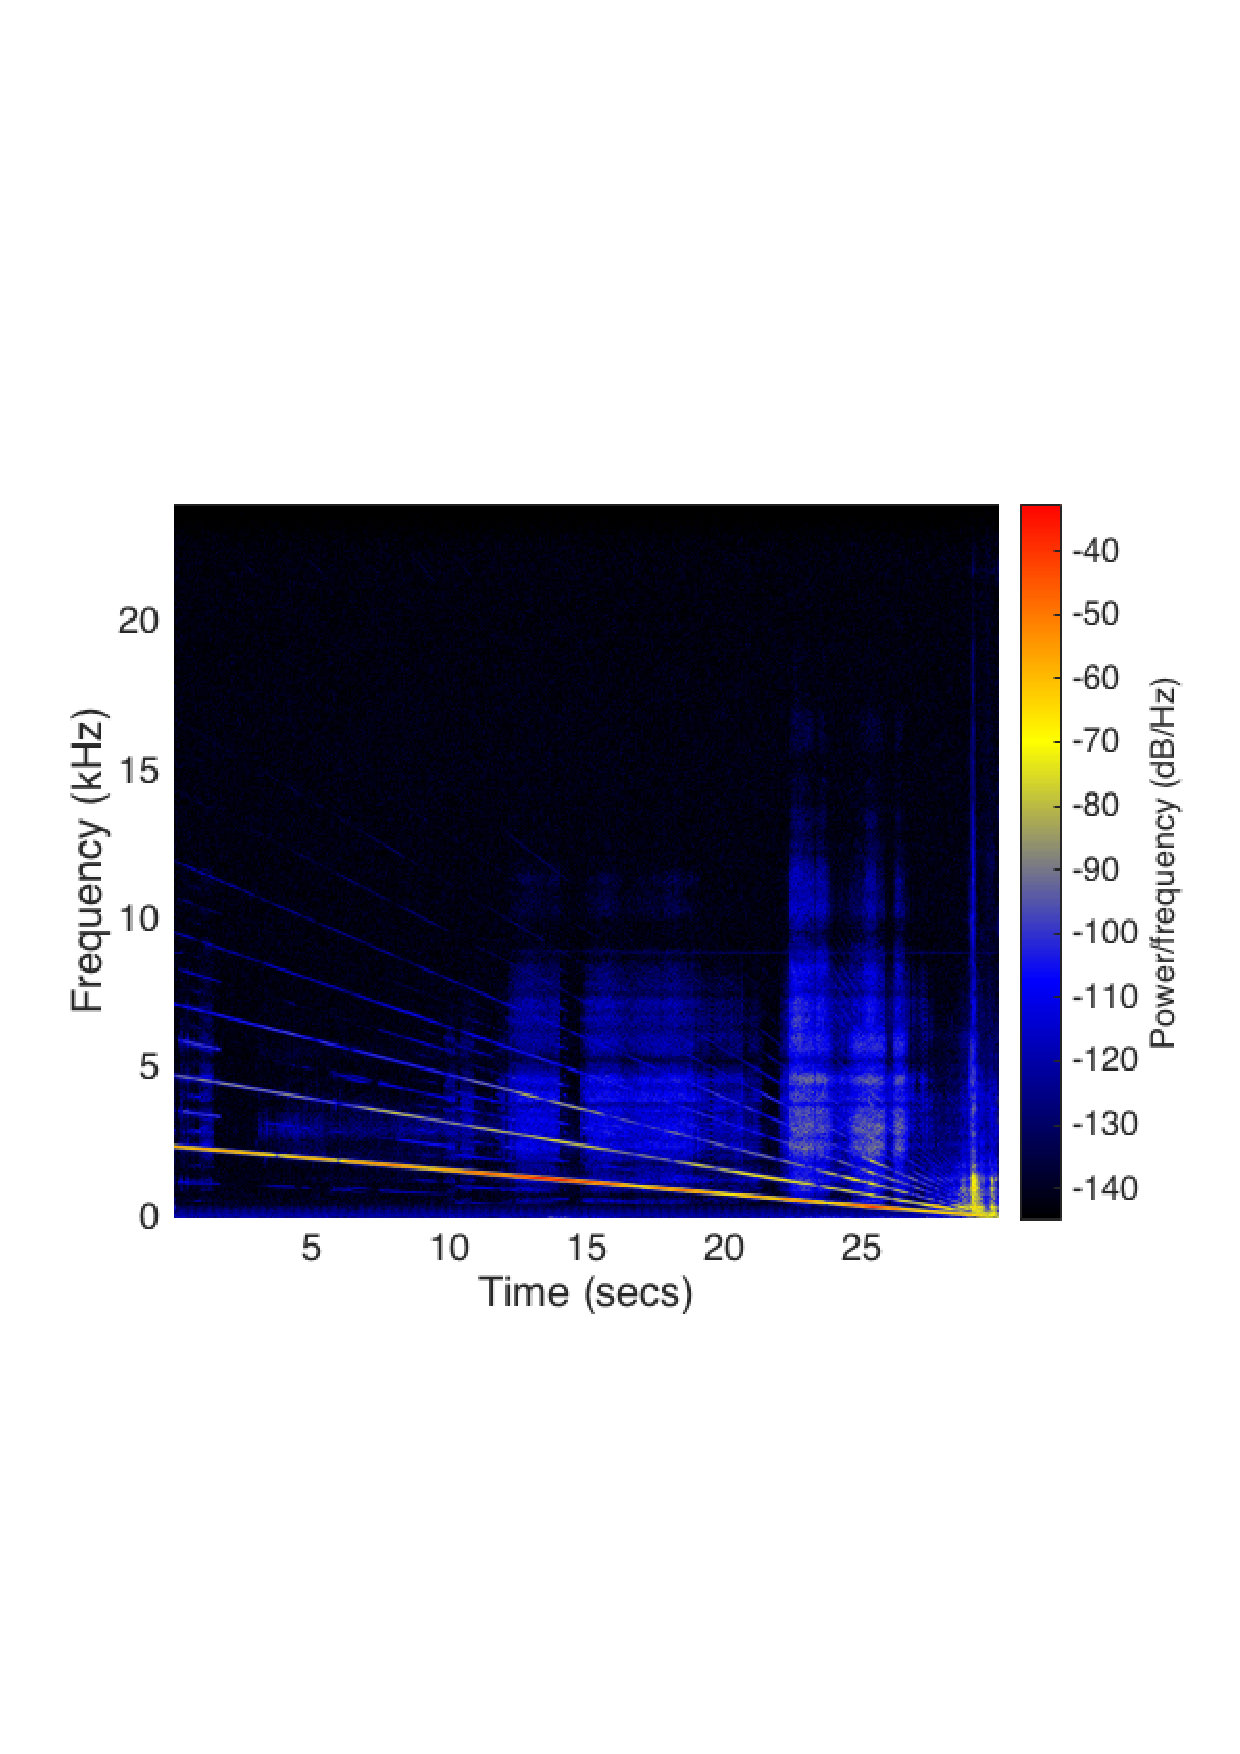
\includegraphics[width=1\textwidth]{figures/spectrogram_enclosure19.pdf}
	\caption{Enclosure dataset 1.}
	\label{fig:spectrogram_enclosure19}
\end{subfigure}
\caption{The spectrograms of the enclosure dataset 1 and 19. The prominent red line is the sine sweep from 2.4 kHz to 10 Hz while the yellow and blue lines along the red line are harmonic distortion.}
\label{fig:spec_enclosure}
\end{figure} 

It is seen that there is considerately more frequency leak throughout the whole spectrum compared to the spectrogram for the driver and microphone. However the measurements from the driver, enclosure, and microphone is the large amount of frequency leak at very low frequencies seen at after 29 seconds.

This section concludes that amount of distortion increases significantly when the gain is increased too. Also, it can be concluded that there is a frequency leak at lower frequencies on both driver, enclosure, and microphone. 




